\subsection{Sanity}

La scelta di adottare \emph{Sanity} come \emph{Content Management System (CMS)} sarebbe stata dettata dalla necessità di gestire in modo strutturato e flessibile le informazioni aziendali, 
rendendole facilmente accessibili a uno o più agenti intelligenti coinvolti nel progetto. 
In particolare, l’obiettivo sarebbe stato quello di mettere a disposizione dell’agente un corpus di conoscenze coerente, aggiornato e contestualizzato rispetto ai 
contenuti pubblicati da \emph{Comfortzone}, così da garantire risposte più affidabili e pertinenti alle richieste degli utenti.

\emph{Sanity} si sarebbe rivelato particolarmente adatto per la sua natura \emph{headless}, che avrebbe consentito di separare la gestione dei contenuti dalla loro 
presentazione e di esporre i dati tramite \emph{API} dedicate. Tale caratteristica avrebbe permesso di integrare facilmente articoli del \emph{blog}, 
schede prodotto e pagine informative in un backend accessibile programmaticamente, favorendo l’estrazione selettiva di informazioni attraverso query mirate \emph{GROQ} (linguaggio dichiarativo per interrogare documenti di formato \emph{JSON}) e 
sperimentazioni in ambiente di \emph{playground}.

Sfruttando il \emph{playground} e le \emph{API}, sarebbe stato possibile testare diverse strategie di estrazione, \emph{chunking} (suddivisione di testi o dati in parti più piccole (\emph{chunk}) per facilitarne l’elaborazione) e indicizzazione dei contenuti per valutare la soluzione più 
efficace per il \emph{retrieval semantico} dell’agente.

Dal punto di vista operativo, l’utilizzo di \emph{Sanity} avrebbe garantito anche un vantaggio pratico: i team editoriali avrebbero potuto aggiornare i contenuti in autonomia e in tempo reale, 
riducendo la necessità di interventi tecnici e assicurando che le conoscenze a disposizione dell’agente rimanessero allineate con le pubblicazioni ufficiali. Questa flessibilità, 
unita alla facile integrazione con servizi esterni come \emph{pipeline} per la generazione di \emph{embedding} (rappresentazione numerica di parole, frasi o documenti in uno spazio vettoriale) o \emph{webhook} (meccanismo che consente a un’applicazione di inviare automaticamente dati o notifiche a un’altra in tempo reale), avrebbe reso \emph{Sanity} 
coerente con gli obiettivi di sperimentazione rapida, scalabilità e iterazione tipici di un \emph{Proof of Concept}.

In sintesi, \emph{Sanity} avrebbe offerto un equilibrio tra struttura dei contenuti, accessibilità via \emph{API} e praticità operativa, elementi che si sarebbero rivelati 
utili per supportare l’agente conversazionale e le successive valutazioni sul suo impatto funzionale e strategico.

\begin{figure}[H]
    \centering
    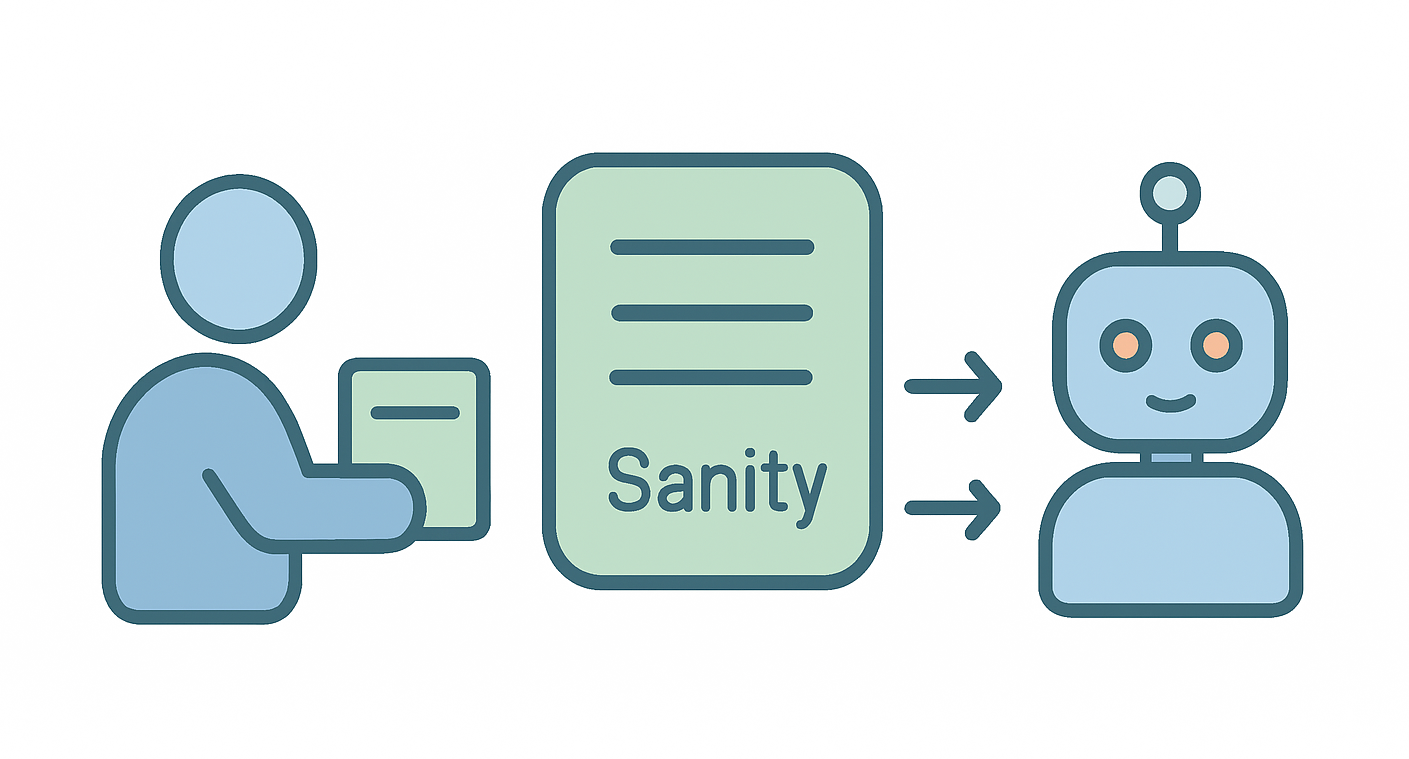
\includegraphics[width=0.8\textwidth]{stage/sanity}
    \caption{Schema illustrativo dell’integrazione dei contenuti tramite Sanity.}
    \label{fig:sanity}
\end{figure}